\documentclass[11pt]{amsart}

% Standard letter size paper with 1inch margins
\usepackage[letterpaper, margin=1in]{geometry}

% Useful packages 
\usepackage{amsmath, amssymb, amsthm, amsaddr}
\usepackage{enumerate, subcaption, graphicx, hyperref}
\usepackage{algorithm}
\usepackage{algpseudocode}
\usepackage{cite}
\usepackage{bm}

\newcommand{\I}{\mathrm{i}}
\DeclareMathOperator{\E}{e}

\title{AMATH 582: Homework 3}
\author{Hunter Lybbert} % first and last name

\address{Applied Mathematics Department, University of Washington, Seattle, WA 
\\ \texttt{hlybbert@uw.edu}}

\date{\today} % you can also just type the date instead of "\today"

\begin{document}

\maketitle

\begin{abstract}
    In this report we convey the results of our survey of supervised machine learning algorithms.
    The MNIST digits dataset was used as a demo task to compare the performance for each of the supervised ML algorithms. We made use of the Ridge Regression Classifier, K-Nearest Neighbors, and Linear Discriminant Analysis. As well as other methods not discussed in class such as Random Forest Classifier and a Gradient Boosted Classifier. Descriptions of the methods, their implimentations, and results are given.
\end{abstract}

\section{Introduction and Overview}\label{sec:Introduction} \textbf{TODO: update this}

\section{Theoretical Background}\label{sec:theory} \textbf{TODO: update this}

Let's get into the actual implementation now.

\section{Algorithm Implementation and Development}\label{sec:algorithms} \textbf{TODO: update this}

As more of an exploratory step we performed an analysis of how much information or energy is retained in our data matrix given a certain number of components are retained in the PCA transformation, see Figure \ref{fig:f0} for a visualization of the percent of energy preserved by a given number of PCA components.

\begin{figure}[h]
	\centering
	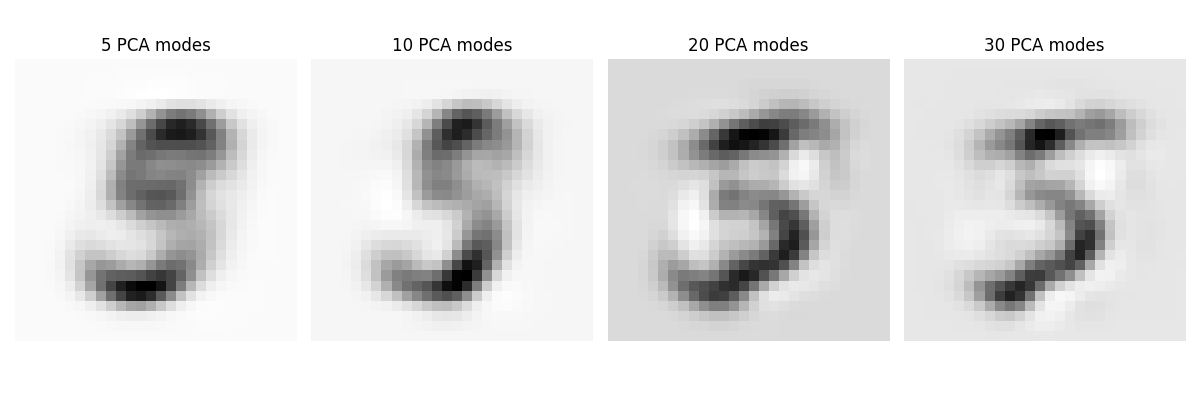
\includegraphics[width=.5\textwidth]{../visualizations/digit_reconstruction.png}
 	\caption{ \textbf{TODO: update this} An analysis of how much information or energy is retained in our data matrix given a certain number of components are used in the PCA transformation.}\label{fig:f0}
\end{figure}

See Figure \ref{fig:f1} for the visuals described.

\begin{figure}[h]
    \centering
    \begin{subfigure}{0.4\textwidth}
        \centering
        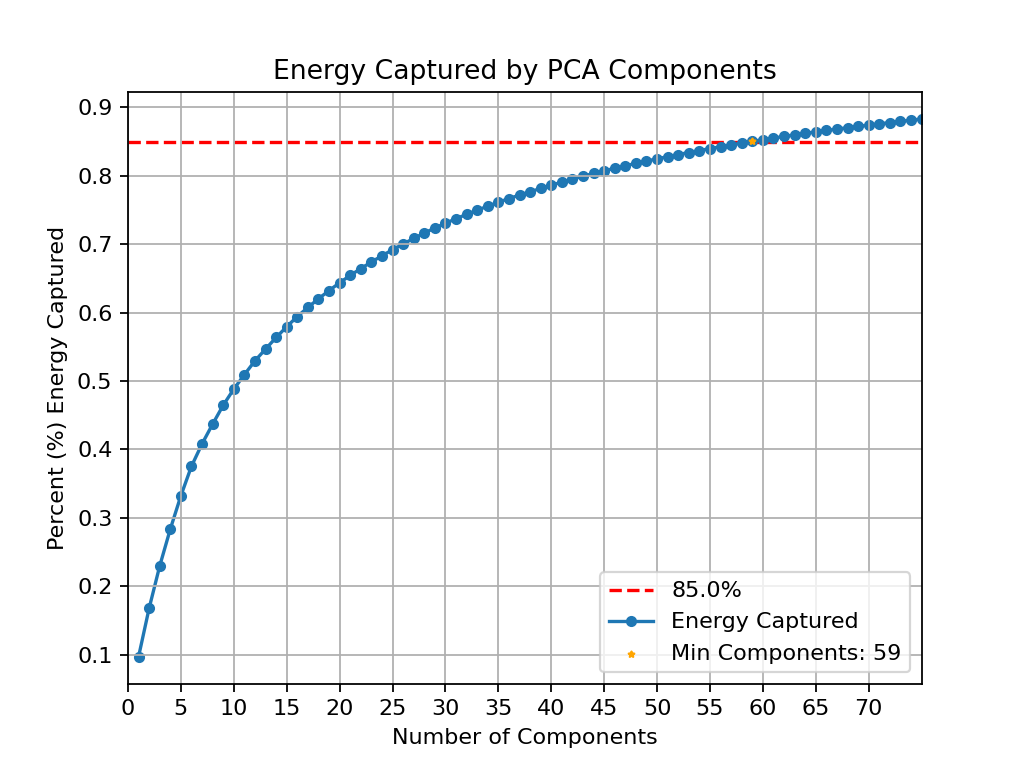
\includegraphics[width=\textwidth]{../visualizations/energy_by_components.png}
        \label{fig:image1}
    \end{subfigure}
    %\hspace{1mm}
    \begin{subfigure}{0.4\textwidth}
        \centering
        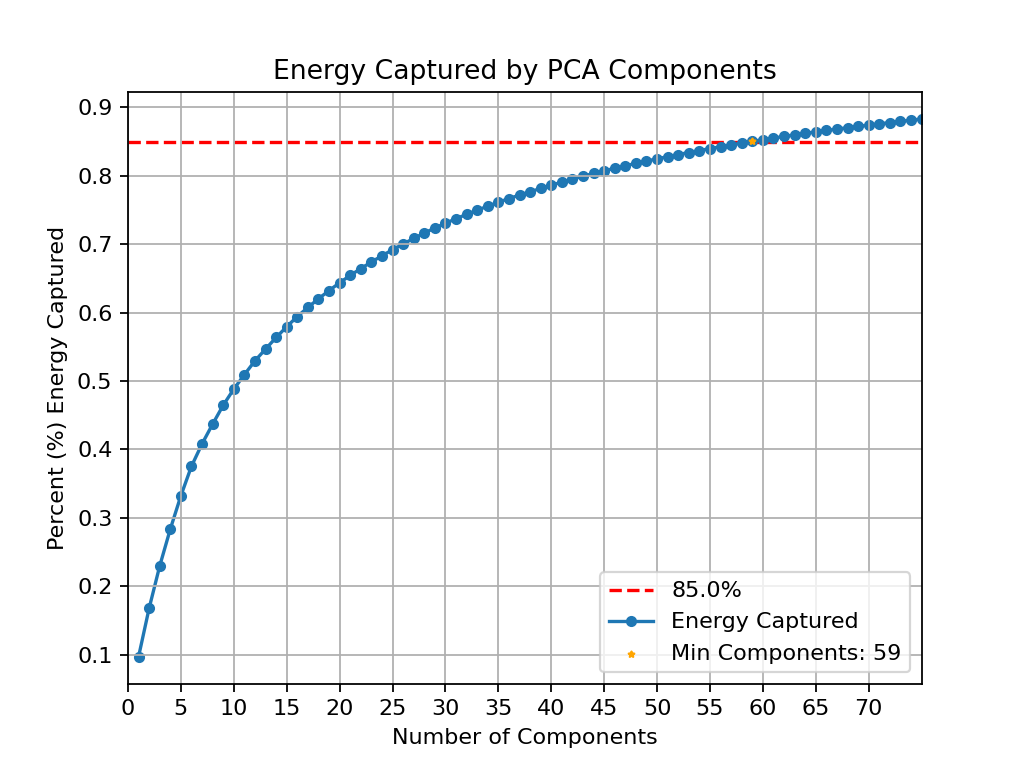
\includegraphics[width=\textwidth]{../visualizations/energy_by_components.png}
        \label{fig:image2}
    \end{subfigure}
    \caption{ \textbf{TODO: update this} We have visualized the lower dimensional projection of the robot movement data in both 2 and 3 dimensions.
    The projected data points (frames from the movement samples) are colored according to movement types.}
    \label{fig:f1}
\end{figure}

 sklearn's \textbf{ClassifierMixin} and \textbf{BaseEstimator} classes.
See code for further details.

\section{Computational Results}\label{sec:results} \textbf{TODO: update this}

\begin{figure}[h]
	\centering
	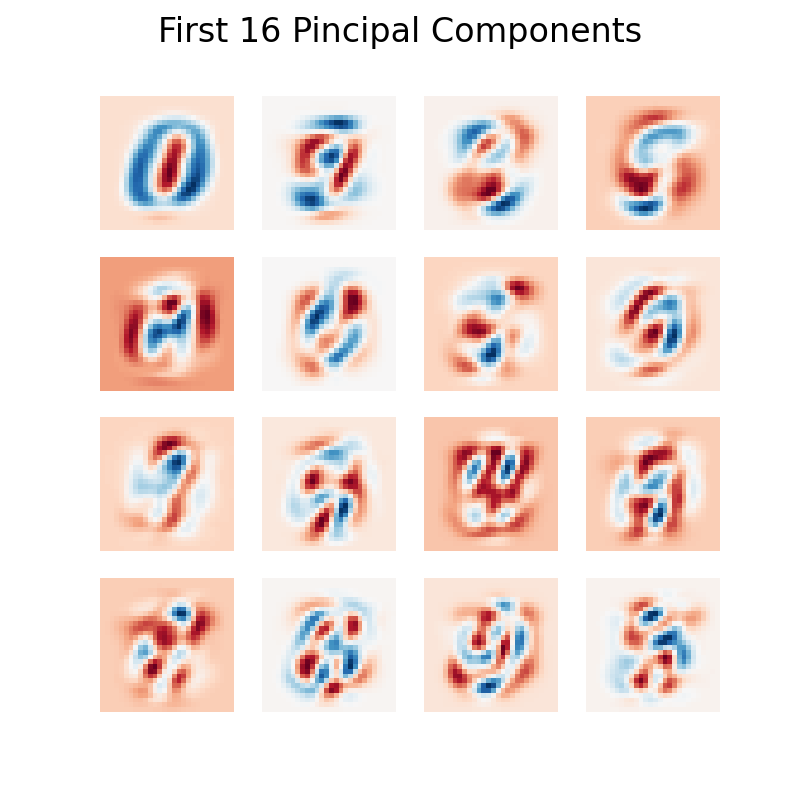
\includegraphics[width=.75\textwidth]{../visualizations/first_16_pincipal_components.png}
 	\caption{ \textbf{TODO: update this} On the left we are looking at the result of projecting the training set into 2 dimensions.
	The centroids we calculated have also been plotted as stars.
	Finally, on the right we have recolored each projected point by which movement type it is classified as using our centroid based classification model.}\label{fig:f2}
\end{figure}

\begin{figure}[h]
	\centering
	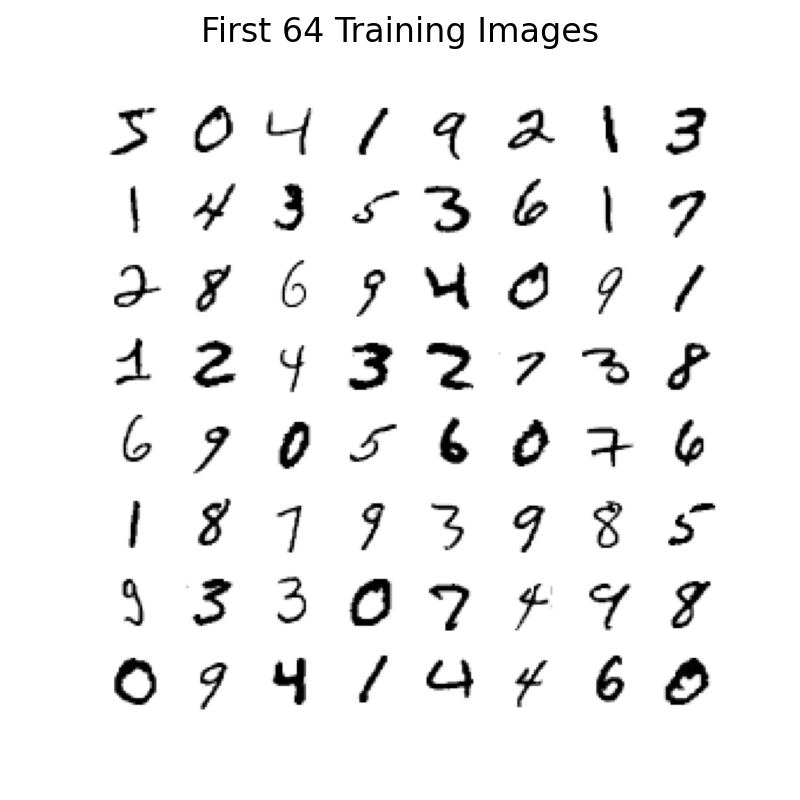
\includegraphics[width=.75\textwidth]{../visualizations/first_64_training_images.png}
 	\caption{ \textbf{TODO: update this} This contains the same information as Figure \ref{fig:f2} with the exception that this is 3d.}\label{fig:f3}
\end{figure}

\section{Summary and Conclusions}\label{sec:conclusions} \textbf{TODO: update this}

\section*{Acknowledgements} \textbf{TODO: update this}

The author is thankful to Jaxon Tuggle, Hailey Sparks, Anja Vogt, Jade Glaister, and Nate Ward.
We would also like to thank Professor Eli Shlizerman for carefully instructing us in class.

\bibliographystyle{abbrv}
\bibliography{references_hw2} % make sure this matches the .bib file for your corresponding document. You also have to maintain your references in the .bib file 

\end{document}
